% --- [ Combined Results ] -----------------------------------------------------

\subsection{Combined Results}
\label{sec:combined_results}

The \textit{combined} control flow recovery results of the Hammock method, the Interval method, and for comparison the theoretical optimum when recovering \textit{2-way conditionals}, \textit{n-way conditionals}, \textit{pre-test loops} and \textit{post-test loops} from the combined test programs of Coreutils and SQLite are presented in figure \ref{fig:total_results_combined}.

The \textbf{Hammock method} correctly recovered $42.16\%$ of the control flow primitives present in the test programs (\textit{true positives}). On average, for every $10$ control flow primitives of the original source code, the Hammock method recovered $3.5$ control flow primitives that were \textit{not} present of the original source code (\textit{false positives}).

The \textbf{Interval method} correctly recovered $74.28\%$ of the control flow primitives present in the test programs (\textit{true positives}). On average, for every $10$ control flow primitives of the original source code, the Interval method recovered $5.9$ control flow primitives that were \textit{not} present of the original source code (\textit{false positives}).

\begin{figure}[htbp]
	\centering
	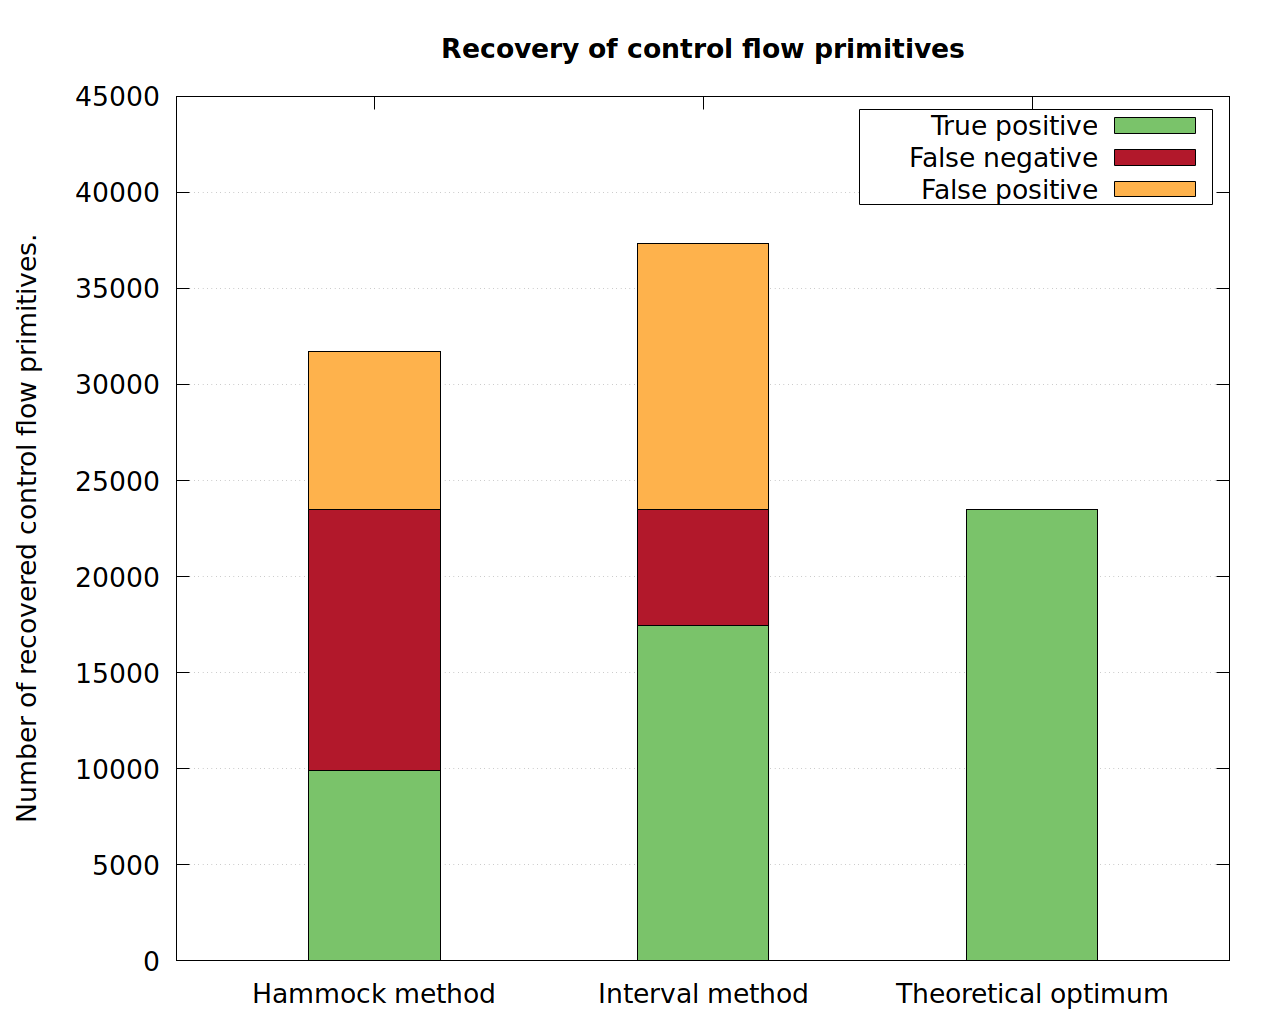
\includegraphics[width=\textwidth]{inc/5_results/results_combined.png}
	\caption{Comparison of control flow recovery results for each method, with the combined results of recovering \textit{2-way conditionals}, \textit{n-way conditionals}, \textit{pre-test loops} and \textit{post-test loops}. The data is based on the combined test programs of Coreutils and SQLite.}
	\label{fig:total_results_combined}
\end{figure}
